% =============================================================================
% =============================================================================
% CAPÍTULO 4 --- COMPONENTE 2: BIOREMPP DATABASE EXPLORER (DBX)
% =============================================================================
% =============================================================================
\chapter{Componente 2: BioRemPP Database Explorer (DBX)}
\label{cap:comp2}

% -----------------------------------------------------------------------------
\section{Motivação e escopo do componente}
\label{sec:c2-motivacao}
% -----------------------------------------------------------------------------

O banco integrado descrito no Capítulo~\ref{cap:comp1} é distribuído em
arquivos CSV e XLSX associados a uma versão publicada. Esse formato preserva
o conteúdo científico, permite sua reutilização programática e mantém o
registro das entidades e relações incorporadas ao banco. Entretanto, a
distribuição por arquivos não oferece, isoladamente, uma camada de consulta
interativa.

A exploração direta desses arquivos exige conhecimento prévio do esquema de
dados e das relações entre compostos, KOs, números EC, reações, vias,
referências institucionais e predições toxicológicas. A estrutura
denormalizada também exige que o pesquisador diferencie o número de linhas das
cardinalidades de cada entidade e reconstrua localmente associações
muitos-para-muitos. Essas operações podem ser executadas em R, Python ou
sistemas de banco de dados, mas dependem da escrita de código e da preparação
do ambiente de análise. O \gls{dbx} fornece uma camada de acesso ao conteúdo integrado sem substituir
os arquivos científicos publicados. A aplicação organiza a evidência em uma
estrutura orientada à consulta e a disponibiliza por uma interface web. O
usuário pode pesquisar entidades, aplicar filtros e percorrer relações entre
compostos, grupos de ortologia KEGG, vias metabólicas, classes químicas,
referências institucionais e predições toxicológicas sem reconstruir
localmente as associações do banco.

A navegação é centrada no composto porque as informações recuperadas pela
interface convergem para as substâncias incluídas no universo institucional do
BioRemPP. Essa organização não reduz todas as evidências a um único
identificador. Os identificadores \gls{cpd} preservam a referência química e
a ligação com as predições toxicológicas, enquanto os identificadores
\gls{ko} conectam os compostos às anotações funcionais do HADEG e do
subconjunto KEGG Degradation. CPD e KO permanecem, portanto, como entidades
complementares de consulta. A aplicação disponibiliza módulos dedicados a compostos, classes químicas,
genes e KOs, vias e toxicidade. Esses módulos permitem consultar registros
individuais e percorrer entidades relacionadas. O componente também reúne
oito análises guiadas que formalizam perguntas sobre amplitude de anotação
funcional, toxicidade predita, classificação institucional e conectividade
entre compostos, KOs e vias. Os filtros e parâmetros dessas análises tornam
explícito o recorte aplicado a cada resultado.

O \gls{dbx} não recebe conjuntos de dados do usuário para processamento. Sua
função é consultar o acervo integrado e versionado. Essa característica o
distingue do \gls{bws}, apresentado no Capítulo~\ref{cap:comp3}, que processa
anotações funcionais submetidas pelo usuário para produzir perfis associados
às amostras analisadas. O Database Explorer opera sobre um conjunto de
referência previamente construído, enquanto o Web Service aplica as relações
do BioRemPP a dados externos. O escopo do \gls{dbx} é exploratório. As associações exibidas representam
registros curados, relações recuperadas de bases públicas e predições
computacionais. Elas sustentam a formulação de hipóteses e a priorização de
entidades para análises posteriores, mas não confirmam a degradação de um
composto nem sua toxicidade em condições ambientais.

A presença de uma substância em uma fonte institucional também não constitui
avaliação jurídica ou determinação de risco para um local específico. Da
mesma forma, a ausência de uma relação na interface pode refletir os limites
de cobertura ou a versão das fontes integradas. A interpretação dos resultados
deve considerar a proveniência, a natureza da evidência e os critérios usados
na construção do banco.

% -----------------------------------------------------------------------------
\section{Arquitetura e organização dos dados}
\label{sec:c2-arquitetura}
% -----------------------------------------------------------------------------

O banco integrado é publicado em arquivos CSV e XLSX com estrutura
denormalizada, adequada à distribuição, à preservação e ao processamento
programático. Essa organização mantém no mesmo arquivo as combinações entre
compostos, KOs, números EC, reações, classes químicas e referências
institucionais. Seu uso direto pela aplicação exigiria ler, filtrar e agrupar
essas combinações a cada requisição.

O BioRemPP Database Explorer usa um banco SQLite derivado dos conjuntos
publicados. Essa representação mantém apenas as estruturas necessárias às
consultas da aplicação e permite selecionar, ordenar, agrupar e paginar os
registros sem processar novamente a tabela denormalizada. O formato em arquivo
único também reduz os componentes necessários para disponibilizar o banco no
ambiente de execução. A camada interna de API orquestra o acesso entre a interface web e o SQLite. A
interface envia os parâmetros de busca, filtragem e paginação, enquanto a API
executa as consultas correspondentes e retorna os resultados em estruturas
consumidas pelos módulos da aplicação. O frontend não acessa diretamente o
banco nem processa os arquivos CSV e XLSX.

Antes da inicialização, o servidor verifica a presença do arquivo SQLite e das
tabelas exigidas pela aplicação. O banco é aberto em modo somente leitura, o
que impede alterações durante as consultas. A API organiza o acesso aos dados
por domínio, com operações específicas para compostos, genes e KOs, vias,
toxicidade, metadados e análises guiadas.

\subsection{Construção do banco SQLite}

A construção do SQLite usa como entradas a tabela central BioRemPP, o HADEG,
o subconjunto KEGG Degradation e o ToxCSM. As informações do HADEG e do
subconjunto KEGG Degradation são associadas à tabela central por KO, enquanto
as predições toxicológicas são relacionadas por CPD.

O processo verifica os identificadores necessários às associações e agrupa os
valores distintos de cada entidade. Os registros são reorganizados por
composto, KO, via, referência institucional e endpoint toxicológico. Também
são preservadas as combinações entre composto, KO, número EC, reação, via e
fonte necessárias às páginas de detalhe e às análises guiadas. O SQLite é reconstruído a partir dos conjuntos correspondentes a cada versão
do banco. Após a carga, verificações de consistência comparam as contagens
armazenadas nos resumos por entidade com os registros que lhes dão origem. Os
resultados quantitativos da construção e dessas verificações são apresentados
na Seção~\ref{sec:c2-resultados}. A Figura~\ref{fig:c2-data-architecture} resume o fluxo entre os conjuntos de
entrada, o banco SQLite, a API interna e a interface web.

\begin{figure}[htbp]
\centering
\fbox{
    \parbox{0.92\textwidth}{
        \centering

        \textbf{Conjuntos de entrada}\\[0.4em]
        BioRemPP central
        \quad HADEG
        \quad KEGG Degradation
        \quad ToxCSM

        \vspace{0.6em}
        $\downarrow$

        \vspace{0.4em}
        \textbf{Associação por KO e CPD}\\
        verificação dos identificadores e agrupamento dos registros

        \vspace{0.6em}
        $\downarrow$

        \vspace{0.4em}
        \textbf{Banco SQLite}\\
        resumos por entidade, mapeamentos e relações contextuais

        \vspace{0.6em}
        $\downarrow$

        \vspace{0.4em}
        \textbf{API interna}\\
        busca, filtragem, ordenação, paginação e análises guiadas

        \vspace{0.6em}
        $\downarrow$

        \vspace{0.4em}
        \textbf{Interface web}\\
        exploradores, páginas de detalhe e visualizações

        \vspace{0.8em}
    }
}
\caption{Arquitetura de dados do BioRemPP Database Explorer. Os conjuntos de
entrada são associados por KO ou CPD e reorganizados em um banco SQLite. A
API interna consulta esse banco e fornece os resultados apresentados pela
interface web. \todo{ELABORAR DIAGRAMA}} 
\label{fig:c2-data-architecture}
\end{figure}

\todo{ELABORAR DIAGRAMA}

Os arquivos publicados e o SQLite atendem a finalidades distintas. Os
arquivos CSV e XLSX preservam e distribuem o conteúdo integrado, enquanto o
SQLite fornece uma representação compacta para as operações da aplicação.
Como o banco de consulta pode ser reconstruído a partir das entradas
versionadas, ele não substitui o artefato científico depositado.

\subsection{Organização dos dados e consulta pela API}

O banco SQLite contém estruturas voltadas a quatro tipos de operação:
consultas por entidade, recuperação de associações, reconstrução do contexto
funcional e acesso às predições toxicológicas. Essa organização evita
recalcular, durante cada consulta, as agregações presentes na tabela
denormalizada.

A Tabela~\ref{tab:c2-data-groups} resume a função desses grupos. Os nomes
completos das tabelas, os campos, os tipos e os índices permanecem registrados
na documentação oficial do projeto.

\begin{table}[htbp]
\centering
\caption{Grupos de dados usados pelo BioRemPP Database Explorer.}
\label{tab:c2-data-groups}
\small
\begin{tabularx}{\textwidth}{@{}p{3.8cm}X@{}}
\toprule
\textbf{Grupo} & \textbf{Função na aplicação} \\
\midrule

Resumos por entidade
& Mantêm uma representação por composto, KO ou via e as contagens usadas em
buscas, filtros e ordenações. \\

Mapeamentos entre entidades
& Registram as associações entre compostos, símbolos gênicos, vias e
referências institucionais. \\

Contexto funcional
& Preserva as combinações entre CPD, KO, atividade enzimática, número EC,
reação, via e fonte. \\

Predições e metadados
& Armazena os valores por combinação composto--endpoint e as informações de
identificação e proveniência associadas ao CPD. \\

\bottomrule
\end{tabularx}
\end{table}

Os resumos por entidade fornecem os campos usados nas listagens e nos filtros
da interface. Para os compostos, esses campos incluem nome, classe química e
contagens de KOs, vias e referências institucionais. A classe química funciona
como atributo de exibição, agrupamento e filtragem; ela não participa das
associações funcionais estabelecidas por KO ou CPD.

As associações entre compostos, KOs, vias e referências institucionais são
mantidas em estruturas próprias. O contexto das associações funcionais
preserva as combinações necessárias para recuperar números EC, reações,
atividades enzimáticas e vias relacionadas a cada composto. As predições
toxicológicas permanecem organizadas por composto e endpoint.

A Figura~\ref{fig:c2-relational-model} apresenta uma visão conceitual dessas
associações. Campos auxiliares e estruturas exclusivas da implementação foram
omitidos.

\begin{figure}[htbp]
\centering
\fbox{
    \parbox{0.88\textwidth}{
        \centering

        \textbf{KOs e anotações funcionais}

        \vspace{0.5em}
        $\updownarrow$

        \vspace{0.5em}
        \textbf{Composto}\\
        CPD, nome, classe química e contagens associadas

        \vspace{0.5em}

        $\swarrow$
        \hspace{4em}
        $\downarrow$
        \hspace{4em}
        $\searrow$

        \vspace{0.5em}

        \textbf{Vias}
        \hspace{3em}
        \textbf{Referências}
        \hspace{3em}
        \textbf{Toxicidade}

        \vspace{0.5em}

        associações por KO
        \hspace{2em}
        fontes institucionais
        \hspace{2em}
        endpoints por CPD

        \vspace{0.8em}
    }
}
\caption{Organização conceitual das consultas no banco SQLite. O composto
constitui o principal ponto de navegação, com associações a KOs, vias,
referências institucionais e endpoints toxicológicos. \todo{ELABORAR DIAGRAMA}}
\label{fig:c2-relational-model}
\end{figure}

Durante a execução, a API consulta exclusivamente o SQLite em modo somente
leitura. As operações são organizadas segundo os módulos da aplicação e
retornam apenas os registros necessários à página solicitada. Os arquivos de
origem não são carregados nem transformados durante essas requisições.

Os arquivos CSV e XLSX preservam o banco integrado para distribuição e
reutilização. O SQLite sustenta as consultas da aplicação, e a API controla o
acesso a essa representação. Cada formato permanece associado à função para a
qual foi produzido.

% -----------------------------------------------------------------------------
\section{Exploração e análises guiadas}
\label{sec:c2-exploracao}
% -----------------------------------------------------------------------------

O BioRemPP Database Explorer oferece duas modalidades complementares de
consulta ao banco integrado. Os módulos de exploração permitem selecionar a
entidade de interesse e combinar critérios de busca, filtragem e ordenação. As
análises guiadas, por sua vez, organizam perguntas previamente definidas e
aplicam procedimentos analíticos específicos a compostos, vias, genes e KOs.

Ambas as modalidades consultam a mesma representação SQLite e preservam a
navegação entre entidades relacionadas. A partir das listagens, o usuário pode
acessar páginas de detalhe que reúnem as associações disponíveis para o
registro selecionado. Essa organização permite iniciar a consulta por uma
entidade química, funcional ou toxicológica e prosseguir pelas relações
mantidas no banco.

\subsection{Módulos de exploração}

A interface organiza a consulta em cinco módulos, definidos pela unidade
representada na listagem principal: compostos, classes químicas, genes e KOs,
vias e toxicidade. Os módulos compartilham operações de busca, filtragem,
ordenação e acesso ao registro detalhado, mas apresentam recortes compatíveis
com a natureza da entidade consultada.

A Tabela~\ref{tab:c2-explorer-modules} resume a unidade de consulta, os
principais critérios de seleção e as relações recuperadas em cada módulo. Os
campos completos das interfaces permanecem descritos na documentação oficial
da aplicação.

\begin{table}[htbp]
\centering
\caption{Módulos de exploração do BioRemPP Database Explorer.}
\label{tab:c2-explorer-modules}
\footnotesize
\begin{tabularx}{\textwidth}{
    @{}
    p{2.4cm}
    p{2.8cm}
    p{4.7cm}
    X
    @{}
}
\toprule
\textbf{Módulo}
& \textbf{Unidade de consulta}
& \textbf{Critérios de seleção}
& \textbf{Relações recuperadas} \\
\midrule

Compostos
& Composto identificado por CPD
& Nome ou CPD, classe química, via, símbolo gênico, referência institucional
e intervalos de contagens.
& KOs, símbolos gênicos, vias, números EC, reações, referências
institucionais e predições toxicológicas. \\

Classes químicas
& Classe associada aos compostos
& Busca pelo nome da classe e seleção dos registros correspondentes.
& Compostos apresentados sob a mesma classe e respectivas medidas derivadas. \\

Genes e KOs
& KO, com símbolo e nome gênico associados
& Busca por KO, símbolo ou nome gênico e intervalo do número de compostos.
& Compostos, vias, atividades enzimáticas e anotações funcionais associadas. \\

Vias
& Combinação entre via e fonte
& Fonte de anotação, nome da via e intervalos de contagens.
& Compostos, KOs e símbolos gênicos associados à via selecionada. \\

Toxicidade
& Combinação entre composto e endpoint
& Grupo de endpoints, endpoint, categoria predita, classe química e intervalo
do valor numérico.
& Predição referente ao endpoint e ligação com o registro do composto. \\

\bottomrule
\end{tabularx}
\end{table}

O módulo de compostos constitui o ponto de entrada para consultas iniciadas
por uma substância específica. Cada registro corresponde a um CPD e apresenta
seu nome, sua classe química e medidas derivadas das associações disponíveis.
Os critérios de seleção permitem restringir o conjunto por anotações
funcionais, vias, referências institucionais e atributos químicos.

A página de detalhe reúne os KOs, símbolos gênicos, números EC, reações e vias
associados ao composto. O mesmo registro apresenta as referências
institucionais e as predições toxicológicas disponíveis, mantendo separadas
informações de natureza funcional, institucional e preditiva. A
Figura~\ref{fig:c2-compounds-explorer} apresenta uma captura representativa
desse módulo.

\begin{figure}[htbp]
\centering
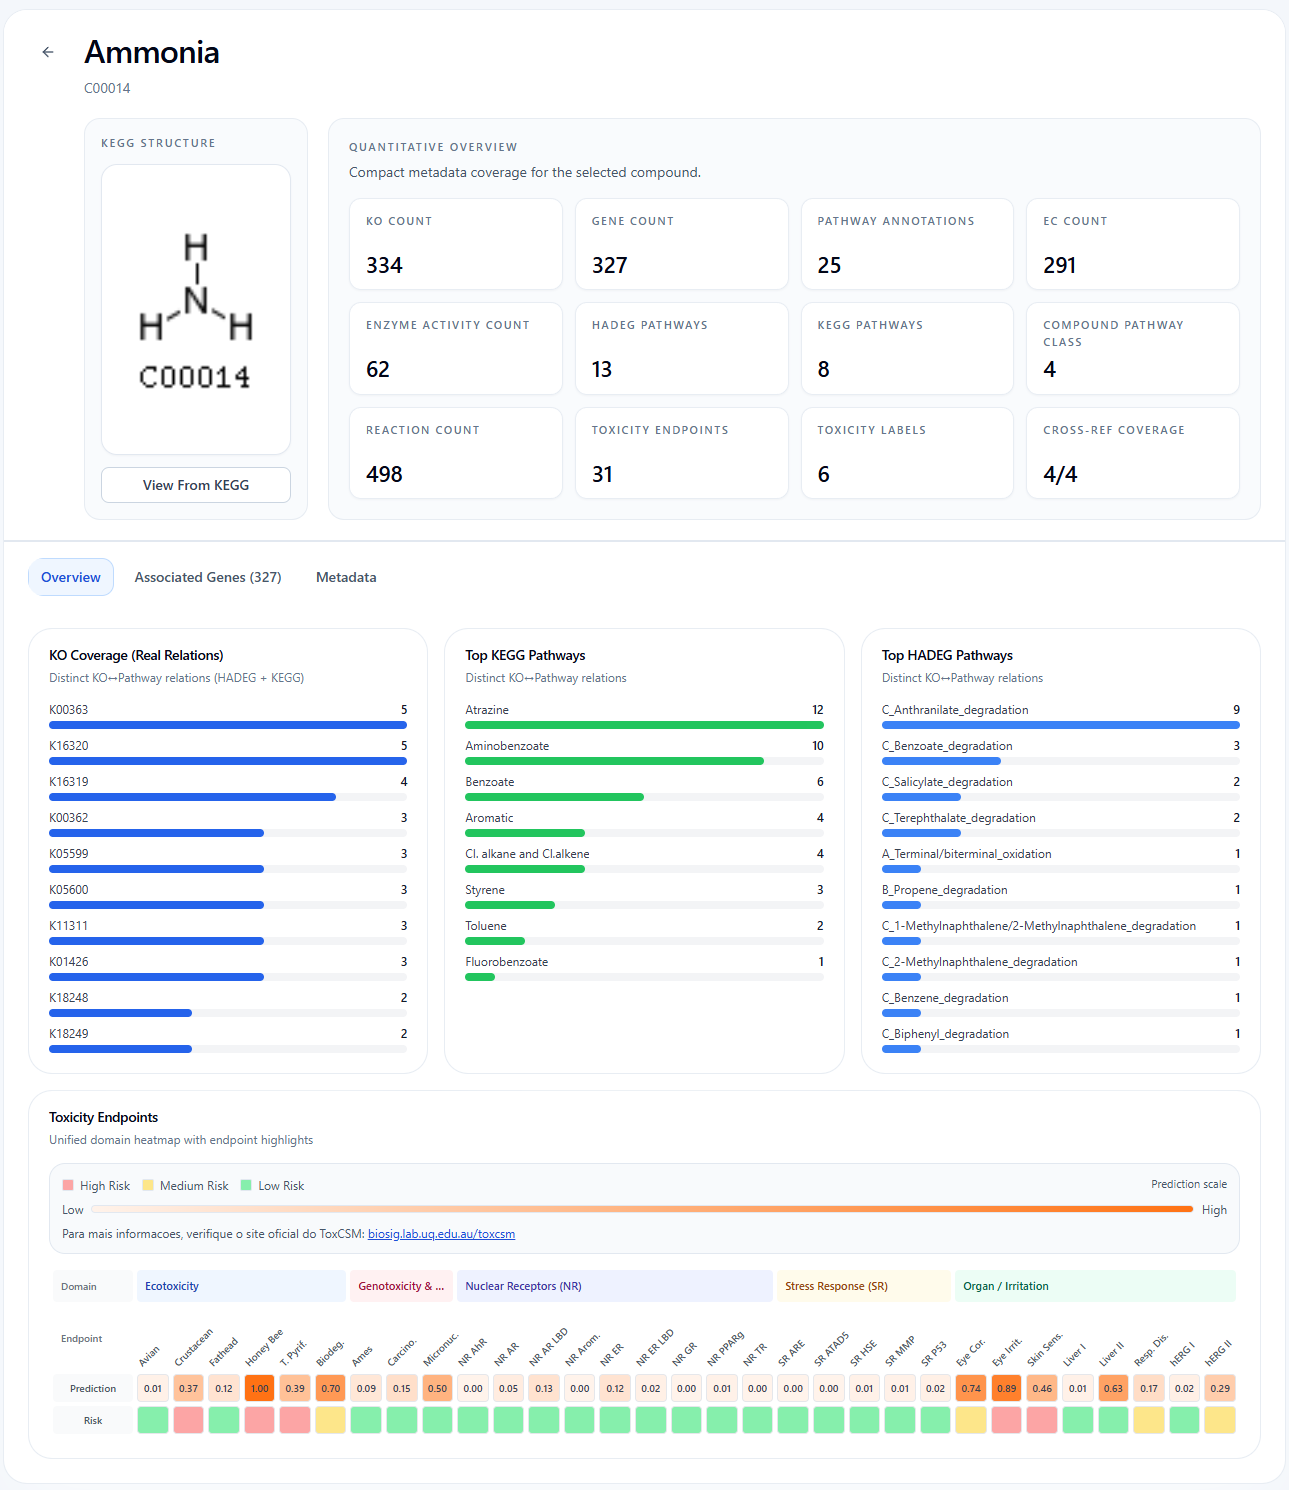
\includegraphics[width=\textwidth]
{figures/chapter_04/fig_04_compounds_explorer.png}
\caption{Módulo de exploração de compostos. A interface reúne critérios de
busca e filtragem com a listagem dos compostos e o acesso ao registro
detalhado de cada CPD.}
\label{fig:c2-compounds-explorer}
\end{figure}

O módulo de classes químicas organiza os compostos segundo o atributo de
classe apresentado pela interface. Essa perspectiva permite delimitar um
conjunto de substâncias antes da consulta aos respectivos registros
individuais. A classe é empregada na apresentação, no agrupamento e na
filtragem dos compostos, sem participar da definição das associações
funcionais estabelecidas por CPD e KO. A seleção de uma classe recupera os compostos apresentados sob o mesmo
rótulo e permite prosseguir para suas páginas de detalhe. A
Figura~\ref{fig:c2-compound-classes-explorer} exemplifica essa forma de
consulta.

\begin{figure}[htbp]
\centering
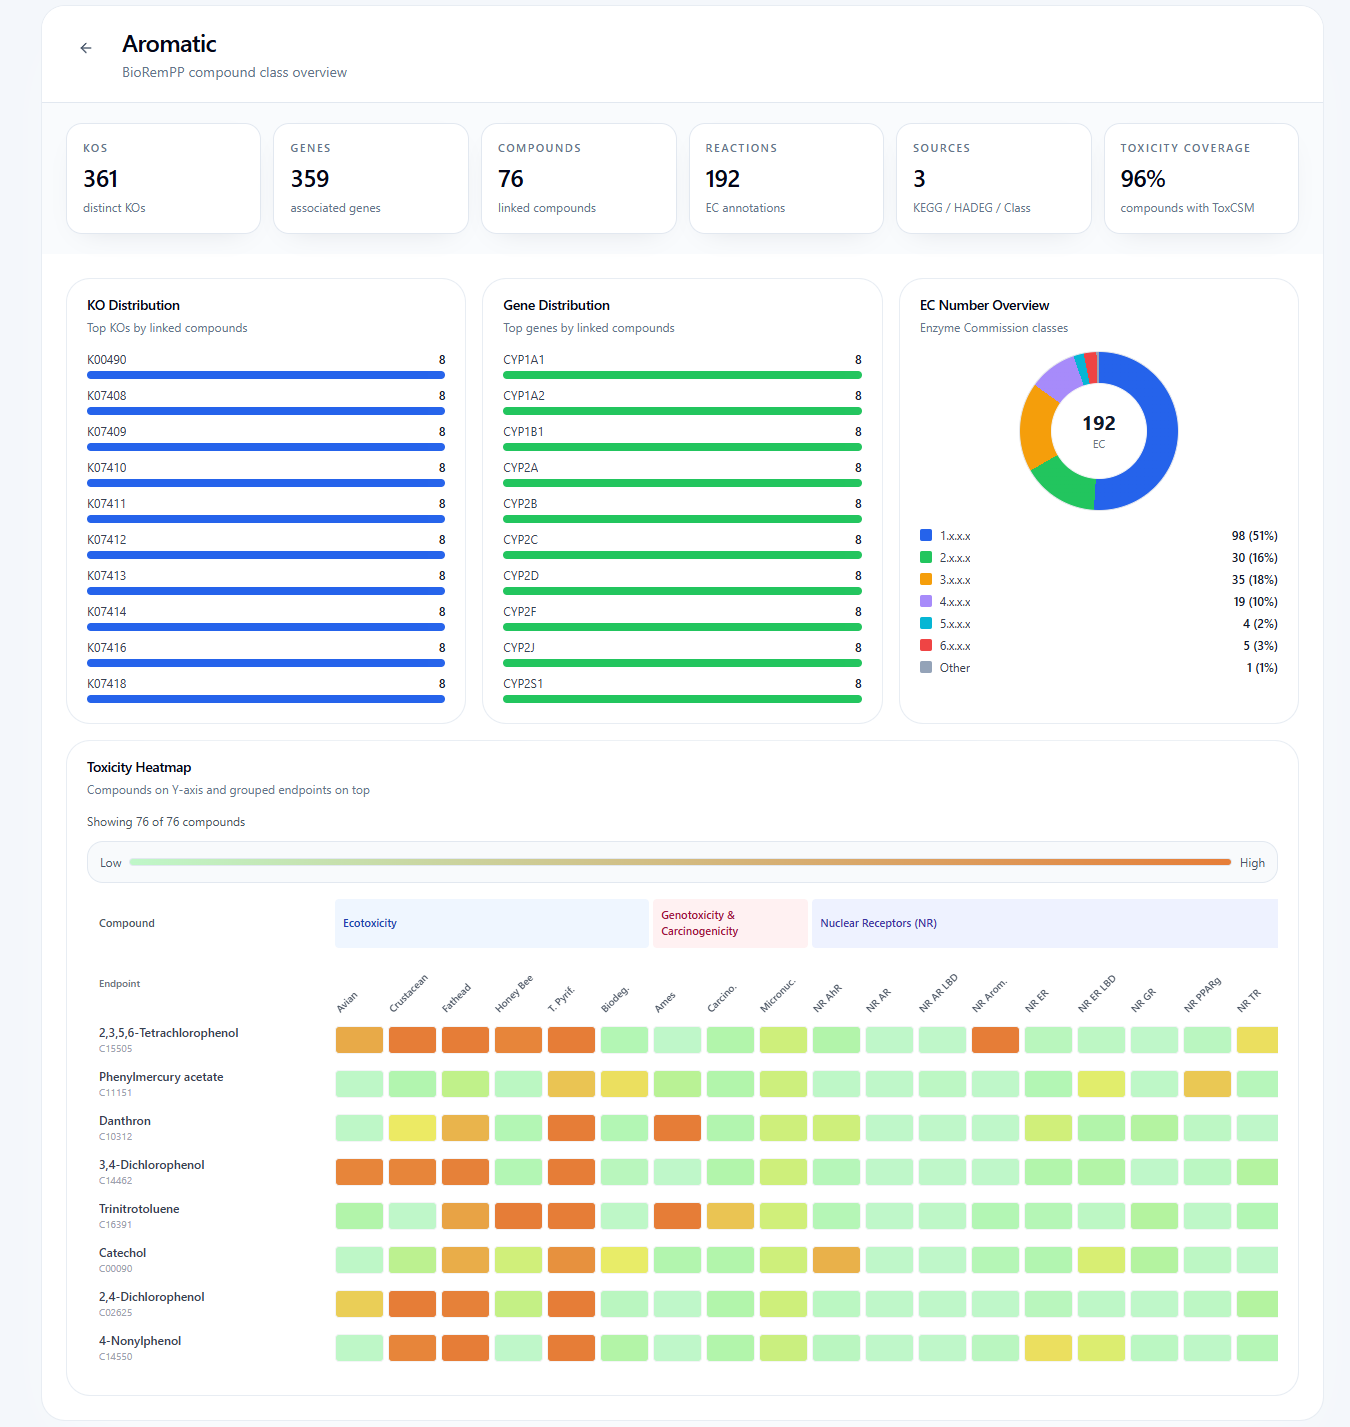
\includegraphics[width=\textwidth]
{figures/chapter_04/fig_04_compound_classes_explorer.png}
\caption{Módulo de exploração de classes químicas. A interface apresenta as
classes empregadas no agrupamento dos compostos e permite acessar os
registros correspondentes.}
\label{fig:c2-compound-classes-explorer}
\end{figure}

O módulo de genes e KOs permite iniciar a consulta por uma entidade funcional.
O KO constitui o identificador principal do registro, enquanto o símbolo e o
nome gênico fornecem descrições associadas. A listagem apresenta medidas
derivadas do número de compostos e vias relacionados a cada KO. A página de detalhe recupera os compostos, as vias, as atividades enzimáticas
e os números EC associados ao registro. As contagens apresentadas descrevem a
conectividade observada no banco e não representam expressão gênica, atividade
enzimática ou relevância metabólica. A
Figura~\ref{fig:c2-genes-ko-explorer} apresenta a organização desse módulo.

\begin{figure}[htbp]
\centering
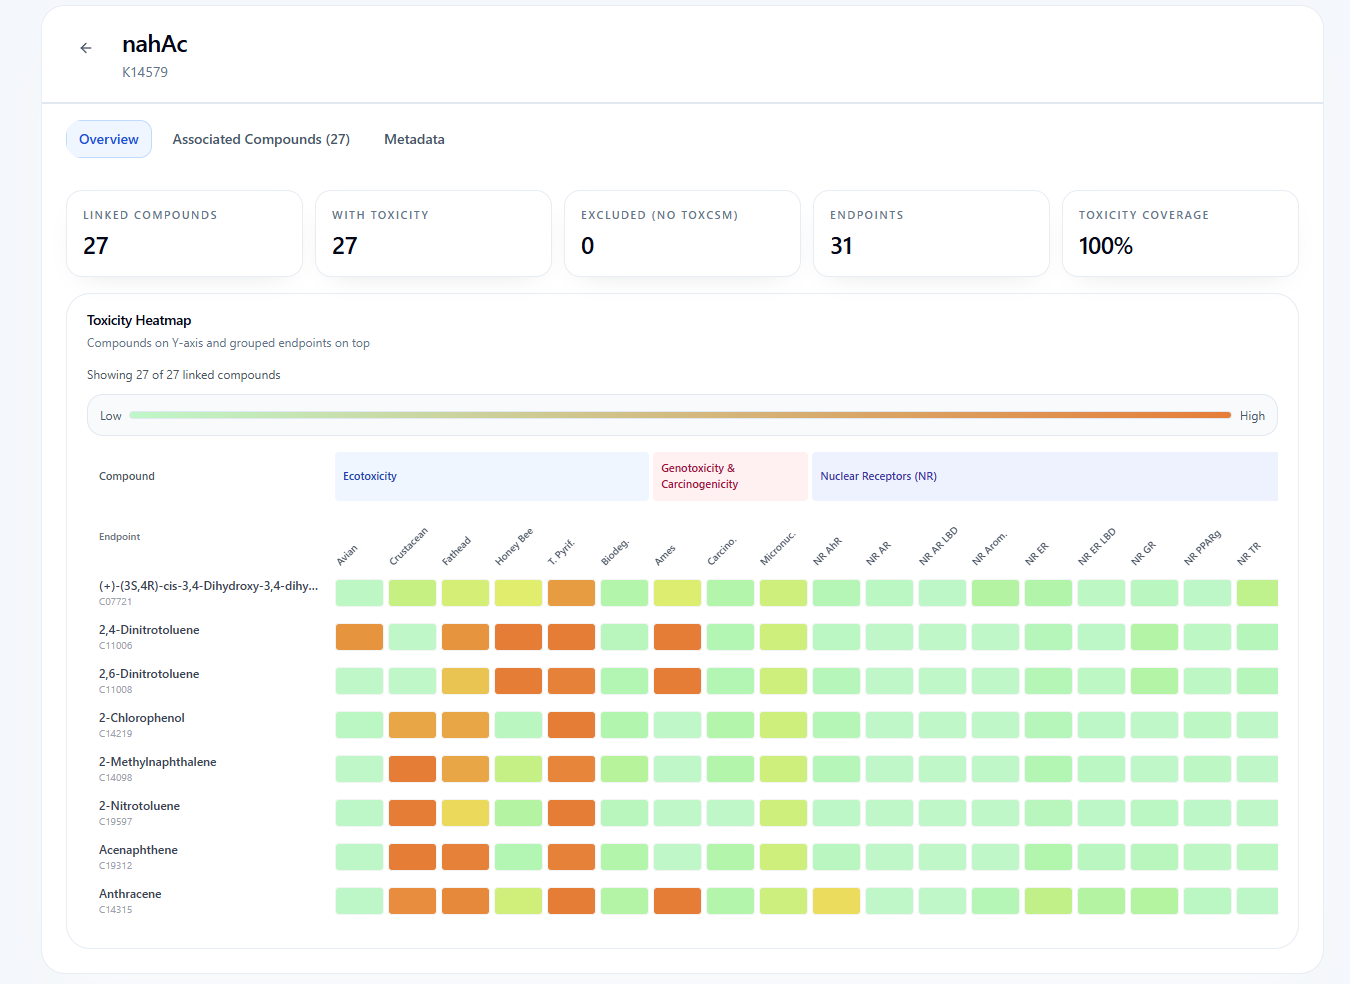
\includegraphics[width=\textwidth]
{figures/chapter_04/fig_04_genes_ko_explorer.png}
\caption{Módulo de exploração de genes e KOs. A interface permite consultar
grupos de ortologia KEGG e recuperar os compostos, as vias e as anotações
funcionais associadas.}
\label{fig:c2-genes-ko-explorer}
\end{figure}

O módulo de vias mantém a fonte de anotação como parte da identificação do
registro. Essa distinção permite consultar separadamente as vias provenientes
do HADEG, do subconjunto KEGG Degradation e das categorias adicionais
incorporadas à representação da aplicação, sem pressupor equivalência entre
seus critérios de organização. Para cada via, a interface apresenta medidas derivadas das associações com
compostos e anotações funcionais. A página de detalhe recupera os compostos e
KOs relacionados ao registro selecionado. Essas contagens não correspondem à
completude da via, ao fluxo metabólico ou à atividade dos seus componentes. A
Figura~\ref{fig:c2-pathways-explorer} exemplifica a consulta por via e fonte.

\begin{figure}[htbp]
\centering
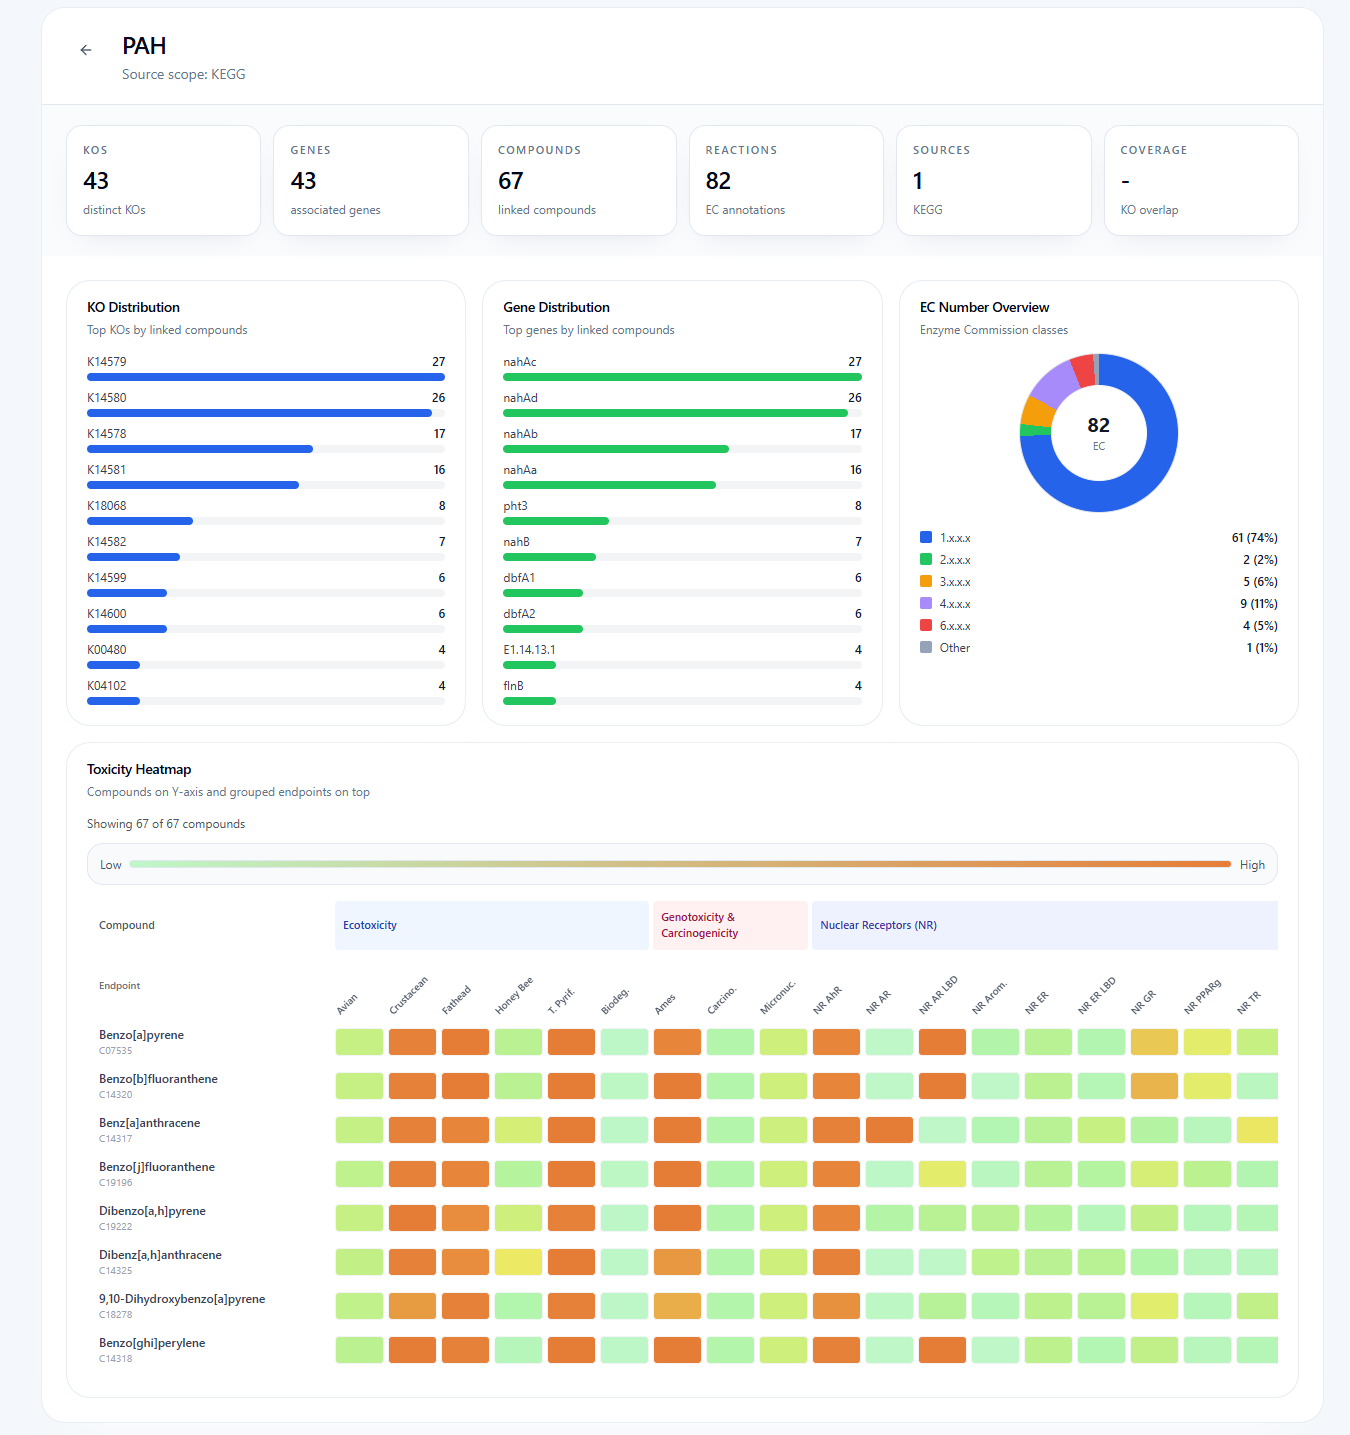
\includegraphics[width=\textwidth]
{figures/chapter_04/fig_04_pathways_explorer.png}
\caption{Módulo de exploração de vias. A interface preserva a fonte de
anotação e permite recuperar os compostos e KOs associados à via
selecionada.}
\label{fig:c2-pathways-explorer}
\end{figure}

O módulo de toxicidade adota a combinação entre composto e endpoint como
unidade de consulta. Os registros podem ser delimitados por grupo de
endpoints, endpoint específico, categoria predita, classe química e intervalo
numérico. A interpretação dos valores permanece condicionada ao endpoint
selecionado, pois os descritores representam propriedades toxicológicas
distintas. Cada resultado mantém a ligação com o CPD correspondente, o que permite
prosseguir para as informações funcionais e institucionais associadas ao
composto. Os valores apresentados resultam de modelos preditivos e não
equivalem a medidas experimentais de toxicidade. A
Figura~\ref{fig:c2-toxicity-explorer} apresenta uma consulta representativa
desse módulo.

\begin{figure}[htbp]
\centering
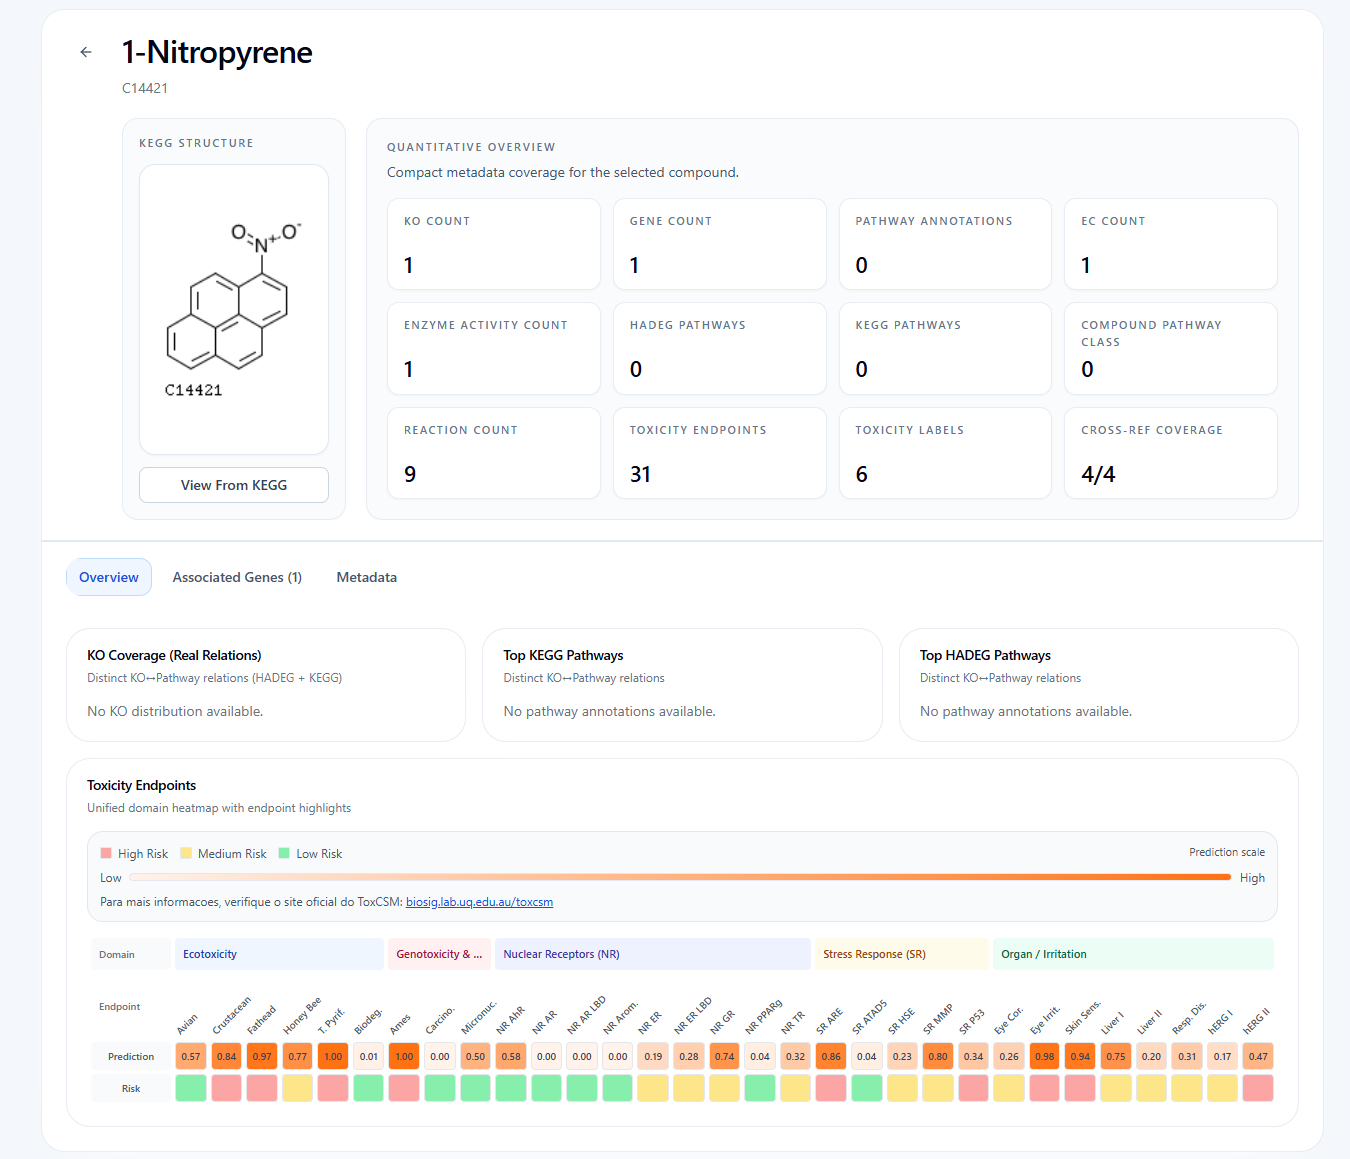
\includegraphics[width=\textwidth]
{figures/chapter_04/fig_04_toxicity_explorer.png}
\caption{Módulo de exploração de toxicidade. A interface organiza as
predições por composto e endpoint e preserva o vínculo com o registro do CPD
correspondente.}
\label{fig:c2-toxicity-explorer}
\end{figure}

A navegação entre as listagens e as páginas de detalhe conecta os cinco
módulos. Um composto recuperado por classe química ou endpoint toxicológico
pode ser examinado por suas associações com KOs e vias. De modo recíproco, uma
consulta iniciada por KO ou via pode conduzir aos compostos relacionados. Essa
navegação mantém a unidade de consulta de cada módulo e utiliza as associações
materializadas no banco SQLite.

\subsection{Análises guiadas}

Os módulos de exploração permitem combinar livremente os critérios de
consulta. As análises guiadas complementam essa modalidade ao formalizar oito
perguntas recorrentes sobre o banco. Para cada pergunta, são definidos a
unidade analisada, os parâmetros, a métrica principal, a ordenação e a forma
de apresentação dos resultados. Cada caso de uso possui uma especificação declarativa em YAML. Essa
especificação registra a pergunta analítica, o conjunto consultado, os
parâmetros aceitos e a operação aplicada. O mesmo arquivo define os elementos
de apresentação, incluindo as medidas resumidas, a visualização, as colunas da
tabela e as orientações para interpretação.

A estrutura compartilhada separa a definição da análise de sua apresentação
na interface. A API recebe o identificador do caso de uso e os parâmetros
selecionados, executa a consulta correspondente sobre o SQLite e retorna uma
resposta com estrutura comum. Essa resposta reúne o escopo da consulta, os
filtros ativos, as medidas resumidas, os dados da visualização e a tabela
paginada.

A Figura~\ref{fig:c2-guided-structure} sintetiza a relação entre a
especificação YAML, a execução pela API, o banco SQLite e a resposta
apresentada ao usuário. As receitas SQL permanecem associadas aos mesmos casos
de uso e documentam as operações necessárias à reprodução das consultas.

\begin{figure}[htbp]
\centering
\fbox{
    \parbox{0.92\textwidth}{
        \centering

        \textbf{Especificação YAML do caso de uso}\\
        pergunta, conjunto, parâmetros, métrica, saída e interpretação

        \vspace{0.6em}
        $\downarrow$

        \vspace{0.4em}
        \textbf{API de análises guiadas}\\
        resolução dos parâmetros e execução da consulta

        \vspace{0.6em}
        $\downarrow$

        \vspace{0.4em}
        \textbf{Banco SQLite}

        \vspace{0.6em}
        $\downarrow$

        \vspace{0.4em}
        \textbf{Resposta compartilhada}\\
        escopo, medidas resumidas, visualização e tabela paginada

        \vspace{0.8em}

        \textbf{Receita SQL associada}\\
        tabelas, junções, filtros, agregações e ordenação
    }
}
\caption{Organização dos casos de uso das análises guiadas. A especificação
YAML define a pergunta, os parâmetros e a apresentação dos resultados; a API
executa a consulta correspondente no SQLite; e a receita SQL documenta a
operação sobre a mesma versão do banco. \todo{ELABORAR DIAGRAMA}}
\label{fig:c2-guided-structure}
\end{figure}

Os oito casos de uso são distribuídos em três grupos. UC1--UC4 usam o composto
como unidade principal; UC5 e UC6 organizam os resultados por via; e UC7 e UC8
partem de símbolos gênicos e dos KOs associados. A
Tabela~\ref{tab:c2-guided-use-cases} apresenta a pergunta, a operação e o
limite interpretativo de cada análise.

\begin{table}[htbp]
\centering
\caption{Casos de uso disponíveis no módulo de análises guiadas.}
\label{tab:c2-guided-use-cases}
\scriptsize
\begin{tabularx}{\textwidth}{
    @{}
    p{0.65cm}
    p{1.65cm}
    p{3.45cm}
    p{4.35cm}
    X
    @{}
}
\toprule
\textbf{ID}
& \textbf{Entrada}
& \textbf{Pergunta analítica}
& \textbf{Métrica e resultado}
& \textbf{Limite de interpretação} \\
\midrule

UC1
& Composto
& Quais compostos apresentam maior amplitude de anotação funcional por KO?
& Ordenação pela contagem de KOs distintos, com gráfico de barras e tabela.
& A contagem descreve a amplitude das anotações disponíveis e não confirma
degradação ou eficiência de remediação. \\

UC2
& Composto e endpoint
& Quais compostos apresentam os maiores valores toxicológicos preditos no
contexto selecionado?
& Ordenação pelo valor de um endpoint ou pelo maior valor dentro de um grupo,
com mapa de calor e tabela.
& Os valores dependem do endpoint selecionado e não constituem medidas
experimentais ou classificação independente de perigo. \\

UC3
& Composto
& Quais compostos combinam maior amplitude de anotação gênica e maior valor
toxicológico predito?
& Gráfico de dispersão entre \texttt{gene\_count} e a medida toxicológica,
com limiares do percentil 75 calculados no conjunto filtrado.
& Os quadrantes são relativos ao recorte analisado; \texttt{gene\_count}
representa a amplitude da anotação disponível, não o desempenho biológico. \\

UC4
& Composto e referência
& Quais compostos estão presentes nas fontes institucionais selecionadas?
& Filtragem por código de referência, ordenação pela quantidade de fontes e
distribuição por referência.
& A presença indica inclusão na fonte integrada e não substitui a avaliação
do enquadramento jurídico vigente ou da magnitude do risco. \\

UC5
& Via
& Quais vias apresentam o maior número de KOs distintos associados?
& Contagem de KOs por combinação entre via e fonte, com ranking e tabela.
& A contagem não mede completude da via, expressão, atividade enzimática ou
fluxo metabólico. \\

UC6
& Via e endpoint
& Quais vias estão associadas a compostos acima do limiar toxicológico
selecionado?
& Contagem e proporção de compostos acima do limiar, com gráfico de barras,
mapa de calor e tabela.
& A associação depende do endpoint e do limiar selecionado e não demonstra
mecanismo toxicológico atribuído à via. \\

UC7
& Símbolo gênico e KO
& Quais genes estão relacionados ao maior número de compostos distintos?
& Contagem de compostos por símbolo gênico, acompanhada pelo número de KOs,
com ranking e tabela.
& A conectividade no banco não representa expressão, atividade catalítica ou
importância metabólica. \\

UC8
& Gene e endpoint
& Quais genes estão associados a compostos acima do limiar toxicológico
selecionado?
& Contagem de compostos acima do limiar e distribuição dos valores por gene,
com gráfico de barras, boxplot e tabela.
& A relação é associativa e depende das predições do endpoint; não estabelece
causalidade entre o gene e a toxicidade. \\

\bottomrule
\end{tabularx}
\end{table}

As operações de contagem consideram entidades distintas para impedir que a
repetição de linhas na representação integrada aumente artificialmente as
medidas. Nas análises toxicológicas, os registros sem valor disponível são
excluídos da operação, e o endpoint ou grupo de endpoints permanece associado
ao resultado.

As visualizações complementam as tabelas sem modificar a métrica definida para
cada caso de uso. Os rankings são apresentados por gráficos de barras; a
relação entre amplitude de anotação e toxicidade predita utiliza gráfico de
dispersão; e as análises dependentes de endpoints empregam mapas de calor ou
boxplots. A interpretação permanece condicionada ao conjunto filtrado e aos
parâmetros registrados na execução.

Cada caso de uso possui uma consulta SQL correspondente. Essas registram as tabelas consultadas, as junções, os critérios de seleção, as
agregações e a ordenação aplicadas. Desse modo, a consulta pode ser repetida
sobre o banco SQLite da mesma versão e com os mesmos parâmetros, sem depender
da visualização fornecida pela aplicação.

Os arquivos YAML e as receitas SQL são versionados com o código do Database
Explorer. Alterações na pergunta, na métrica, nos parâmetros ou no critério de
ordenação permanecem associadas à versão do software que contém a respectiva
definição.

A Figura~\ref{fig:c2-guided-analysis} apresenta a interface das análises
guiadas em execução. A captura reúne a seleção do caso de uso, os parâmetros
ativos, as medidas resumidas, a visualização e a tabela de resultados,
evidenciando a estrutura compartilhada pelas oito análises.

\begin{figure}[htbp]
\centering
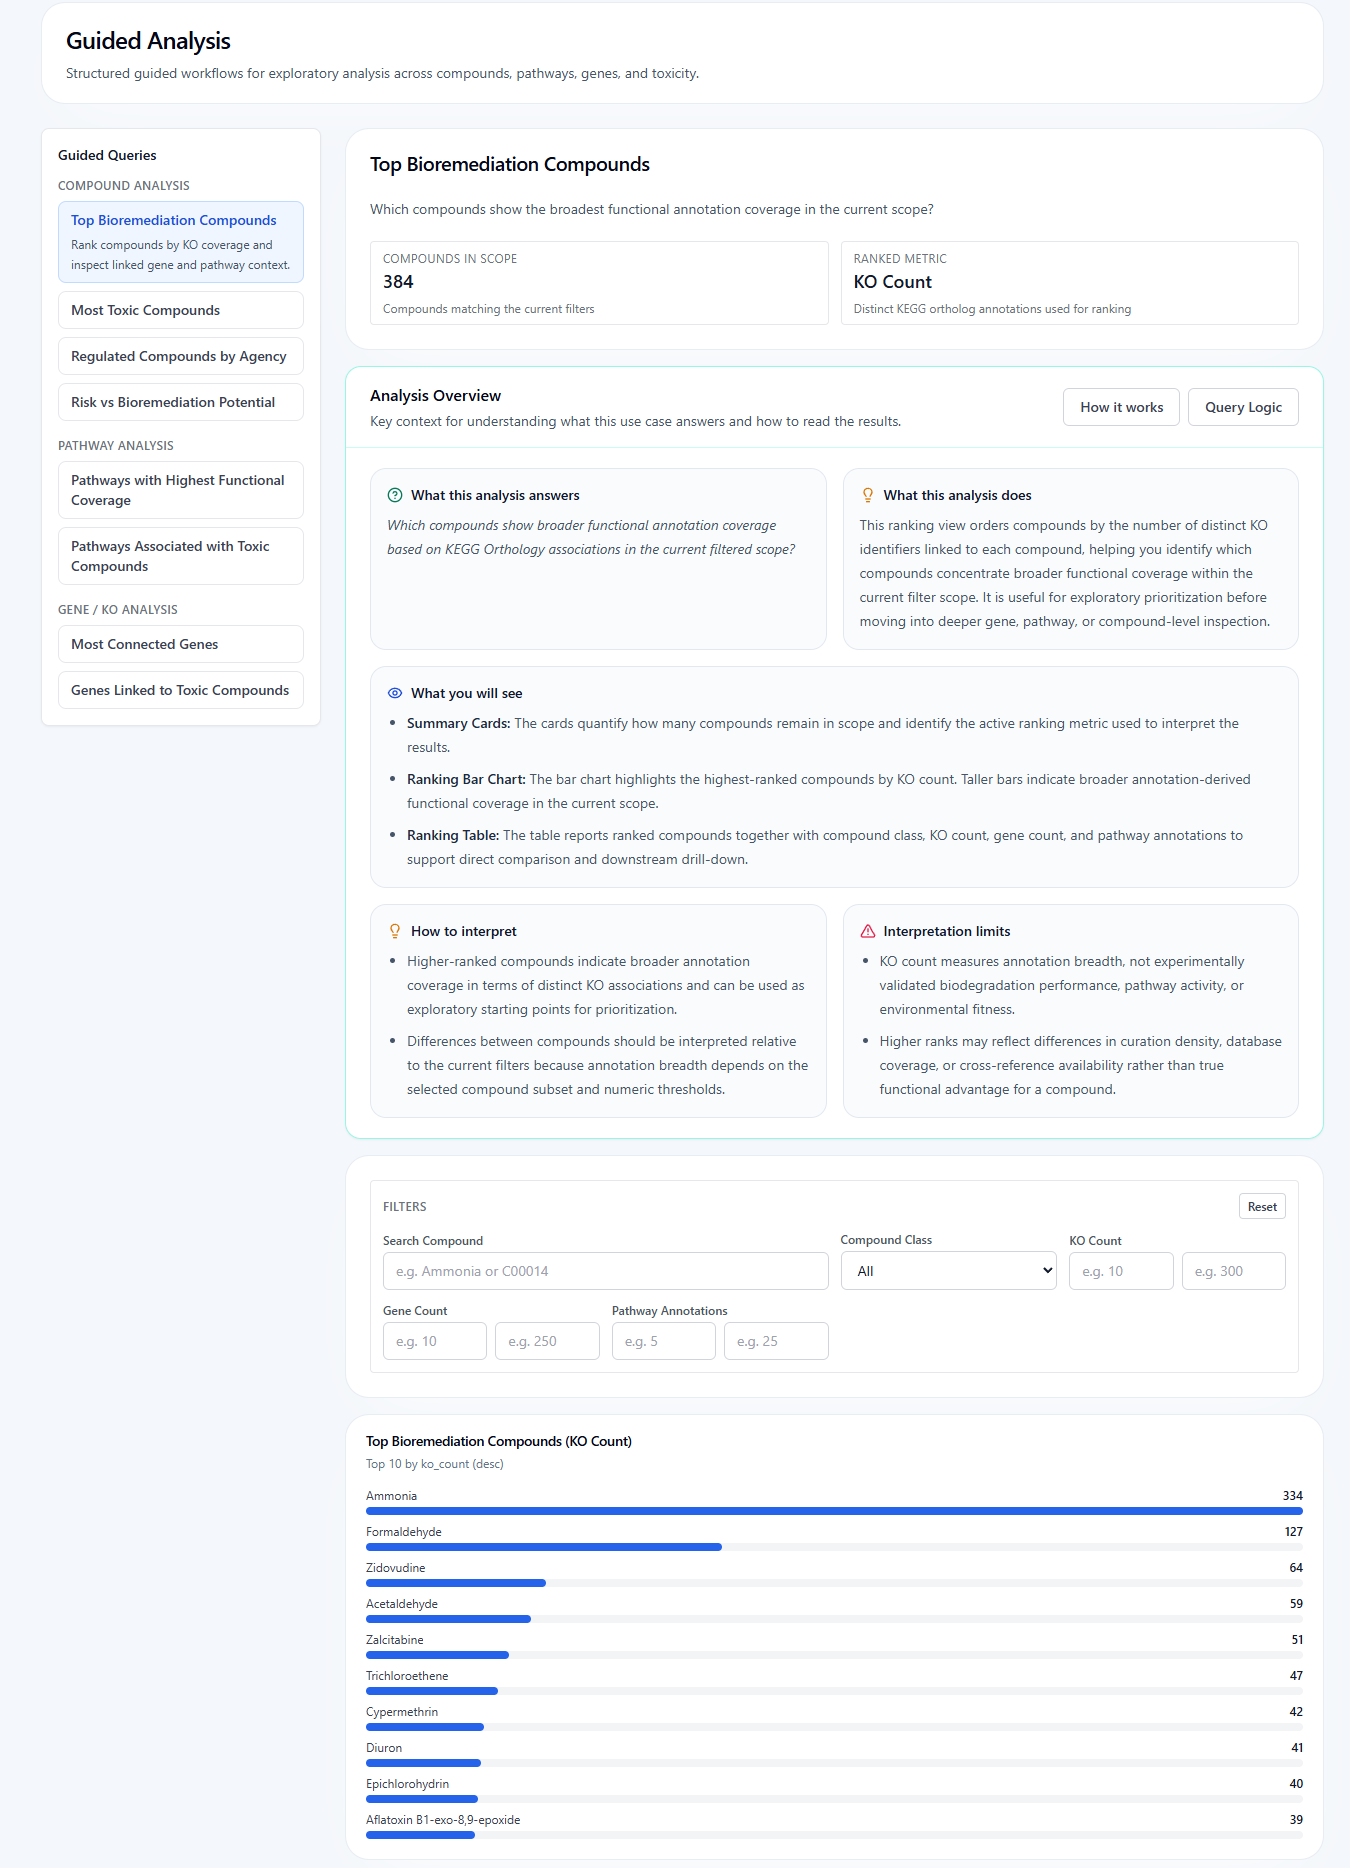
\includegraphics[width=\textwidth]
{figures/chapter_04/fig_04_guided_analysis.png}
\caption{Módulo de análises guiadas do BioRemPP Database Explorer. Cada caso
de uso reúne uma pergunta analítica, parâmetros de consulta, medidas
resumidas, visualização e tabela de resultados sob uma estrutura comum.}
\label{fig:c2-guided-analysis}
\end{figure}

% -----------------------------------------------------------------------------
\section{Resultados do componente}
\label{sec:c2-resultados}
% -----------------------------------------------------------------------------

O BioRemPP Database Explorer foi implementado como ambiente web de consulta à
versão do banco apresentada no Capítulo~\ref{cap:comp1}. Os resultados
compreenderam a implementação do ambiente de consulta, a disponibilização dos
módulos de exploração, a execução das análises guiadas. 

\subsection{Implementação do ambiente de consulta}

A versão avaliada reúne uma interface desenvolvida em React e TypeScript, uma
API interna baseada em Express e um banco SQLite destinado às operações da
aplicação. Esses elementos integram uma configuração conteinerizada que
combina o servidor, a interface compilada e a representação dos dados utilizada
durante a execução.

O banco SQLite contém as 12 tabelas requeridas pelo servidor e ocupa
15,77~MiB. A aplicação acessa esse arquivo em modo somente leitura, e as
consultas não dependem do carregamento dos arquivos CSV e XLSX publicados. O
SQLite constitui, portanto, a representação operacional do conteúdo descrito
no Capítulo~\ref{cap:comp1}, sem substituir os artefatos científicos
disponibilizados para distribuição e reutilização dos dados.

A API interna disponibiliza operações para os domínios de compostos, classes
químicas, genes e KOs, vias, toxicidade, metadados e análises guiadas. Na
avaliação da versão, as requisições aos módulos examinados retornam respostas
válidas e preservam os mecanismos de paginação, filtragem e recuperação das
entidades relacionadas.

\subsection{Módulos de exploração e navegação entre entidades}

Os cinco módulos previstos integram a aplicação: \textit{Compounds},
\textit{Compound Classes}, \textit{Genes / KO}, \textit{Pathways} e
\textit{Toxicity}. As Figuras~\ref{fig:c2-compounds-explorer} a
\ref{fig:c2-toxicity-explorer} apresentam as respectivas interfaces, enquanto
a Tabela~\ref{tab:c2-explorer-modules} sintetiza suas unidades de consulta e
as relações recuperadas.

O módulo de compostos recupera as anotações funcionais, as vias, as referências
institucionais e as predições toxicológicas associadas a cada CPD. O módulo de
classes químicas agrupa os compostos conforme o atributo utilizado na
interface. Os módulos de genes e KOs e de vias iniciam as consultas por
entidades funcionais, enquanto o módulo de toxicidade organiza os resultados
por combinação entre composto e endpoint.

A avaliação verifica a navegação entre as listagens e as páginas de detalhe a
partir das relações retornadas pela aplicação. Os registros de compostos
conduzem aos KOs, às vias e às predições toxicológicas associadas. No sentido
inverso, as consultas iniciadas por KO ou via recuperam os compostos
correspondentes. Os módulos de classes químicas e toxicidade também preservam
o acesso ao registro individual de cada composto.

A verificação examina a correspondência entre as entidades apresentadas nas
listagens e aquelas recuperadas nas páginas de detalhe. Seu escopo não abrange
uma avaliação de usabilidade com participantes nem a mensuração do desempenho
da interface sob carga concorrente.

\subsection{Análises guiadas e reprodutibilidade das consultas}

Foram implementados e executados os oito casos de uso descritos na
Tabela~\ref{tab:c2-guided-use-cases}. Quatro análises adotaram o composto como
unidade principal, duas organizaram os resultados por via e duas partiram de
genes e KOs. Todos os casos retornaram os resultados, as medidas resumidas e
as visualizações definidas nas respectivas configurações.

\begin{table}[htbp]
\centering
\caption{Execução dos grupos de análises guiadas do BioRemPP Database
Explorer.}
\label{tab:c2-guided-execution}
\small
\begin{tabularx}{\textwidth}{@{}p{3.1cm}p{2.5cm}X@{}}
\toprule
\textbf{Grupo}
& \textbf{Casos de uso}
& \textbf{Resultado da execução} \\
\midrule

Compostos
& UC1--UC4
& As quatro análises foram executadas e produziram os resumos, as
visualizações e as tabelas definidos para consultas centradas em compostos. \\

Vias
& UC5--UC6
& As duas análises foram executadas sobre as associações entre vias, KOs,
compostos e predições toxicológicas. \\

Genes e KOs
& UC7--UC8
& As duas análises foram executadas sobre as associações entre símbolos
gênicos, KOs, compostos e valores toxicológicos preditos. \\

\bottomrule
\end{tabularx}
\end{table}

As oito análises seguem a estrutura compartilhada apresentada na
Figura~\ref{fig:c2-guided-structure}. A aplicação processa as configurações
YAML para definir os parâmetros, as medidas resumidas, as visualizações e as
tabelas de cada caso de uso. A API organiza essas informações em um formato
comum, independentemente da entidade adotada como ponto de entrada.

A Figura~\ref{fig:c2-guided-analysis} exemplifica a interface correspondente.
Todos os casos de uso mantêm a mesma organização, composta pela seleção da
análise, definição dos parâmetros, apresentação das medidas resumidas,
visualização e tabela de resultados.

Cada caso de uso permanece associado a uma receita SQL versionada. As oito
receitas operam sobre a mesma versão do banco SQLite e reproduzem as unidades
de análise, os filtros, as agregações, as métricas principais e os critérios de
ordenação definidos pela aplicação. As diferenças relacionadas à paginação ou
à seleção dos campos apresentados permanecem restritas à projeção da resposta e
não modificam as operações analíticas.

A associação entre as especificações YAML e as receitas SQL registra tanto a
configuração utilizada pela interface quanto a consulta executada sobre o
banco. Essa organização possibilita repetir os procedimentos analíticos
independentemente das visualizações apresentadas pelo BioRemPP Database
Explorer.

\subsection{Verificação técnica e disponibilização}

A suíte automatizada executou 172 testes distribuídos em 53 arquivos, sem
falhas. As verificações abrangeram os módulos de exploração, as configurações
das análises guiadas, os componentes de visualização, as funções
compartilhadas e o comportamento esperado da interface.

A verificação de tipos, a análise estática e a compilação da aplicação foram
concluídas sem erros. A cobertura de testes atendeu aos limiares definidos
para linhas, instruções, funções e desvios condicionais. As oito
especificações YAML e as respectivas receitas analíticas também foram
validadas pelos procedimentos automatizados do projeto.

O perfil do banco SQLite foi verificado quanto à presença das estruturas
requeridas, à integridade do arquivo e ao limite de tamanho definido para o
ambiente de execução. A construção da imagem conteinerizada foi concluída, e
os serviços atingiram o estado saudável. As consultas realizadas no
contêiner reproduziram as respostas obtidas no ambiente local para os módulos
avaliados e para os oito casos de uso.

A Tabela~\ref{tab:c2-technical-verification} resume os resultados das
verificações realizadas sobre a versão avaliada.

\begin{table}[htbp]
\centering
\caption{Resultados das verificações técnicas do BioRemPP Database Explorer.}
\label{tab:c2-technical-verification}
\small
\begin{tabularx}{\textwidth}{@{}p{4.1cm}p{2.3cm}X@{}}
\toprule
\textbf{Verificação}
& \textbf{Resultado}
& \textbf{Evidência principal} \\
\midrule

Testes automatizados
& Aprovada
& 172 testes foram aprovados em 53 arquivos. \\

Cobertura de testes
& Aprovada
& Os limiares configurados para linhas, instruções, funções e desvios
condicionais foram atendidos. \\

Verificação de tipos
& Aprovada
& Nenhum erro de tipagem foi identificado. \\

Análise estática
& Aprovada
& Nenhuma violação bloqueante permaneceu no código avaliado. \\

Compilação da aplicação
& Aprovada
& A interface e o servidor foram compilados para o ambiente de produção. \\

Configurações das análises guiadas
& Aprovada
& As oito especificações YAML foram processadas e validadas. \\

Receitas SQL
& Aprovada
& As oito receitas reproduziram as métricas principais das análises
correspondentes. \\

Perfil do banco SQLite
& Aprovada
& O arquivo apresentou as 12 tabelas requeridas, integridade válida e
15,77~MiB. \\

Execução conteinerizada
& Aprovada
& A imagem foi construída, os serviços atingiram estado saudável e as
consultas de verificação retornaram respostas válidas. \\

\bottomrule
\end{tabularx}
\end{table}


Os elementos necessários à reprodução do Database Explorer foram mantidos no
repositório, incluindo o código-fonte, os arquivos de configuração, as
especificações YAML, as receitas SQL, a definição do ambiente conteinerizado e
a documentação. O uso dos identificadores CPD e KO preservou a
correspondência com as entidades adotadas no banco publicado.

O BioRemPP Database Explorer foi disponibilizado em
\url{https://bioinfo.imd.ufrn.br/bioremppdbx/}. O código-fonte encontra-se em
\url{https://github.com/BioRemPP/biorempp-dbx}, e a documentação está
disponível em
\url{https://biorempp-dbx.readthedocs.io/en/stable/}. O código foi distribuído sob a licença Apache~2.0, enquanto os dados
permaneceram disponíveis sob a licença CC~BY~4.0.

% -----------------------------------------------------------------------------
\section{Discussão do componente}
\label{sec:c2-discussao}
% -----------------------------------------------------------------------------

O BioRemPP Database Explorer não acrescenta novas evidências ao banco
integrado, mas modifica as condições de acesso às associações já
estabelecidas. Os arquivos publicados permanecem como referência versionada
para distribuição e reutilização, enquanto a aplicação permite consultar o
mesmo conteúdo sem manipulação direta da tabela central. A contribuição do
componente está na tradução da estrutura integrada em consultas iniciadas por
entidades químicas, funcionais e toxicológicas.

O uso de um banco SQLite atende ao perfil consultivo da aplicação. O
Database Explorer opera sobre dados previamente integrados e não recebe
alterações produzidas pelos usuários durante a execução. A representação
operacional permite aplicar filtros, ordenações, agregações e paginação sem
reprocessar os arquivos CSV e XLSX em cada requisição. A abertura do banco em
modo somente leitura também preserva o conteúdo materializado durante o uso
da interface. A separação entre os arquivos publicados e o SQLite mantém funções distintas
para os dois formatos. Os arquivos CSV e XLSX preservam o conteúdo científico
em uma forma adequada à distribuição, à citação e ao processamento externo. O
SQLite organiza as estruturas exigidas pelas consultas da aplicação e pode ser
reconstruído a partir da versão correspondente dos conjuntos de entrada. A
interface não se torna, portanto, a única forma de acesso ao banco BioRemPP. A API interna restringe o acoplamento entre a interface e a organização física
dos dados. Os módulos enviam os parâmetros da consulta e recebem respostas
estruturadas sem acessar diretamente o arquivo SQLite. Essa separação permite
alterar a apresentação dos resultados sem modificar a representação
científica publicada e concentra no servidor as regras de consulta
compartilhadas pelos diferentes módulos.

A organização dos exploradores por entidade permite formular consultas a
partir de diferentes pontos de entrada. O módulo de compostos parte do CPD,
enquanto os módulos de genes e KOs e de vias iniciam a consulta pela dimensão
funcional. Os módulos de classes químicas e toxicidade acrescentam recortes
voltados, respectivamente, ao agrupamento dos compostos e às predições por
endpoint. Essa organização operacionaliza a complementaridade entre CPD e KO
descrita no modelo do banco. A navegação entre listagens e páginas de detalhe mantém o contexto das
associações recuperadas. Um composto pode ser examinado em relação aos KOs,
vias, números EC, reações, referências institucionais e endpoints associados.
De forma recíproca, uma consulta iniciada por KO ou via permite recuperar os
compostos relacionados. Os módulos funcionam, assim, como diferentes acessos
ao mesmo conjunto de relações, e não como coleções independentes.


As contagens exibidas nos exploradores sintetizam a quantidade de associações
registradas para cada entidade. Elas permitem ordenar resultados e delimitar
conjuntos para inspeção, mas não medem expressão gênica, atividade enzimática,
completude de vias ou eficiência de degradação. Uma contagem elevada indica
maior amplitude de anotação no banco, condicionada às fontes integradas e aos
critérios de curadoria descritos no Capítulo~\ref{cap:comp1}.

As análises guiadas complementam a exploração baseada em filtros livres. Os
oito casos de uso formalizam perguntas recorrentes ao definir a unidade
analisada, os parâmetros aceitos, a métrica calculada e a forma de
apresentação. Essa definição reduz a variação decorrente da composição manual
de filtros e mantém explícito o procedimento aplicado a cada consulta. A implementação declarativa em YAML associa a pergunta analítica aos
parâmetros, às medidas resumidas, à visualização e aos limites de
interpretação. Alterações nesses elementos permanecem vinculadas à versão da
configuração correspondente. A definição da análise fica separada dos
componentes responsáveis por sua apresentação, o que permite distinguir
mudanças no procedimento analítico de modificações exclusivamente de interface.

As receitas SQL associadas aos casos de uso fornecem uma representação
executável das consultas. A repetição dos resultados depende da mesma versão
do SQLite, dos mesmos parâmetros e dos mesmos critérios para valores ausentes,
agregações e ordenação. A receita documenta o procedimento independentemente
da interface, enquanto o YAML registra como esse procedimento é parametrizado
e apresentado no Database Explorer. A reprodução das métricas principais pelas receitas SQL indica
correspondência entre as análises executadas pela aplicação e sua descrição
externa. Diferenças de paginação, seleção de campos ou apresentação de
subconjuntos não modificam necessariamente a operação analítica. Essas
diferenças precisam, contudo, permanecer documentadas quando a saída da
interface for comparada diretamente à consulta completa. Os casos de uso mantêm caráter exploratório. Os rankings baseados em KOs,
símbolos gênicos ou compostos descrevem relações presentes no banco e não
demonstram desempenho biológico. As análises que combinam anotações funcionais
e valores toxicológicos também não estabelecem causalidade entre genes, vias e
toxicidade. Os resultados permitem priorizar registros para inspeção, mas
exigem validação independente antes de sustentar conclusões experimentais.

A interpretação das predições toxicológicas depende do endpoint selecionado.
Cada endpoint descreve uma propriedade distinta e pode apresentar escala,
direção e significado próprios. Seus valores não devem ser combinados como uma
medida única de risco sem justificativa específica. As categorias exibidas
também não substituem ensaios experimentais ou avaliações formais de perigo. Os limiares calculados a partir do conjunto filtrado produzem classificações
relativas ao recorte analisado. No caso da análise que relaciona amplitude de
anotação gênica e toxicidade predita, a posição de um composto depende da
distribuição dos registros incluídos na consulta. A alteração dos filtros pode
modificar os limiares e a distribuição entre os quadrantes, que não
correspondem a classes permanentes dos compostos.

O escopo do Database Explorer permanece restrito à consulta do banco
integrado. O componente não processa dados ômicos submetidos pelos usuários,
não atualiza automaticamente as fontes externas e não realiza avaliação
regulatória individualizada. O processamento de amostras pertence ao serviço
de análise do ecossistema BioRemPP, enquanto decisões regulatórias exigem a
consulta às fontes oficiais e à legislação vigente.


A disponibilização do código-fonte, da documentação, das configurações YAML,
das receitas SQL e do ambiente conteinerizado fornece mecanismos concretos
para reprodução e reutilização. O uso de CPD e KO preserva a correspondência
com identificadores externos, enquanto o versionamento associa as consultas à
versão dos dados e do software. As licenças do código e do banco explicitam as
condições de uso dos respectivos artefatos.

Esses mecanismos apoiam aspectos dos princípios FAIR no escopo do Database
Explorer. A aplicação e a documentação ampliam o acesso ao conteúdo; CPD e KO
favorecem a interoperabilidade; as receitas SQL e as configurações versionadas
permitem repetir as consultas; e as licenças estabelecem as condições de
reutilização.

No ecossistema BioRemPP, o Database Explorer ocupa a camada de consulta direta
ao banco integrado. Os arquivos publicados preservam o conteúdo científico, o
Database Explorer permite examinar suas associações e o serviço de análise
aplica esse conhecimento a dados fornecidos pelos usuários. A contribuição
específica do componente consiste em converter o banco versionado em um
ambiente de consulta por entidades relacionadas, com procedimentos analíticos
explícitos e limites de interpretação definidos.
